% !TEX root = manual.tex
\section{Hypercube}
\label{subsec:tutorial:hypercube}

Although never used at scale in a production system, the generalized hypercube is an important topology to understand, particularly for flattened butterfly and dragonfly.
The (k,n) generalized hypercube is geometrically an N-dimensional torus with each dimension having size k (although dimension sizes need not be equal).
Here we show a (4,2) generalized hypercube (Figure \ref{fig:topologies:hypercubeConnected}).  This would be specified in SST as:

\begin{ViFile}
topology.name = hypercube
topology.geometry = 4 4 
\end{ViFile}
indicating size 4 in two dimensions. 

While a torus only has nearest-neighbor connections, a hypercube has full connectivity within a row and column (Figure \ref{fig:topologies:hypercubeConnected}).
Any switches in the same row or same column can send packets with only a single hop.

\begin{figure}[h!]
\centering
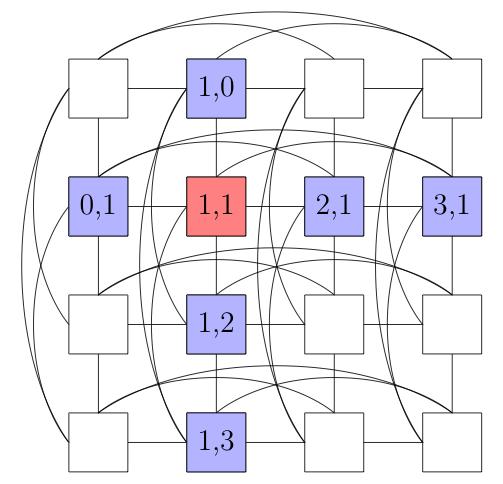
\includegraphics[width=0.5\textwidth]{figures/tikz/hypercube/hypercube_connected.png}
\caption{Hypercube with links and connections within a row/column}
\label{fig:topologies:hypercubeConnected}
\end{figure}

This extra connectivity leads to greater path diversity and higher radix switches.
The cost tradeoff is that each link has lower bandwidth than a torus. 
Whereas a torus has a few fat links connecting switches, a hypercube has many thin links.
A hypercube can have more dimensions and be asymmetric, e.g.

\begin{ViFile}
topology.name = hypercube
topology.geometry = 4 5 6
\end{ViFile}

where now we have full connections within horizontal rows, horizontal columns, and vertical columns.
Here each switch has radix 12 (3 connections in X, 4 connections in Y, 5 connections in Z). 

\subsection{Allocation and indexing}
A hypercube has the same coordinate system as a torus. For example, to create a very specific, irregular allocation on a hyerpcube:

\begin{ViFile}
app1.launch_cmd = aprun -n 5
app1.indexing = coordinate
app1.allocation = coordinate
app1.coordinate_file = coords.txt
\end{ViFile}

and then a coordinate file named \inlineshell{coords.txt}
\begin{ViFile}
5 2
0 0
0 1
1 1
2 0
3 3
\end{ViFile}
The first line indicates 5 entries each with 2 coordinates.
Each line then defines where MPI ranks 0-4 will be placed

\begin{figure}[h!]
\centering
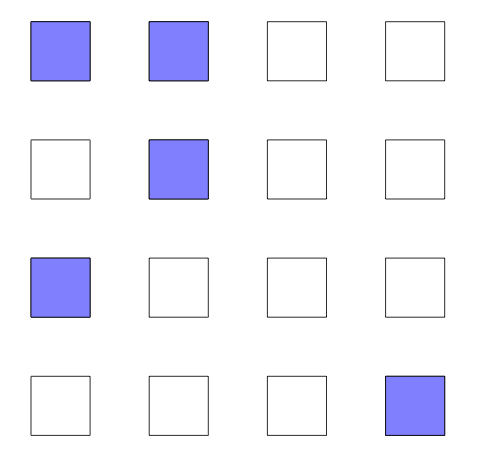
\includegraphics[width=0.5\textwidth]{figures/tikz/hypercube/hypercube_allocation.png}
\caption{Hypercube allocation for given set of coordinates}
\label{fig:topologies:hypercubeAllocation}
\end{figure}

\subsection{Routing}
Hypercubes allow very path-diverse routing because of its extra connections.
In the case of minimal routing (Figure \ref{fig:topologies:hypercubePath}), two different minimal paths from blue to red are shown.
While dimension order routing would rigorously go X then Y, you can still route minimally over two paths either randomly selecting to balance load or routing based on congestion.

\begin{figure}[h!]
\centering
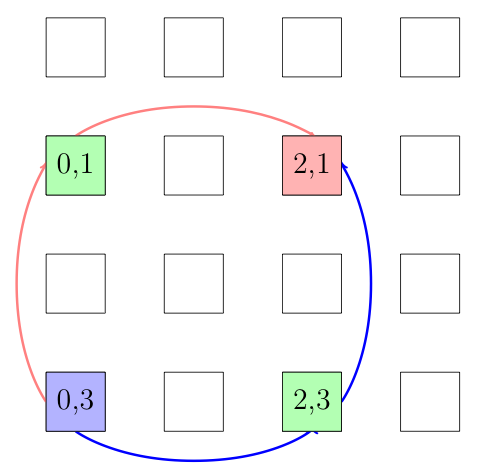
\includegraphics[width=0.5\textwidth]{figures/tikz/hypercube/hypercube_path.png}
\caption{Minimal routing within a hypercube showing path diversity. Packet travels from blue to red, passing through green intermediate switches.}
\label{fig:topologies:hypercubePath}
\end{figure}

To fully maximize path diversity on adversarial traffic patterns, though, path-diverse topologies can benefit from Valiant routing.
Here, rather than directly routing to the final destination, packets first route to random intermediate switches on a minimal path.
Then they route again from the intermediate switch to the final destination also on a minimal path (Figure \ref{fig:topologies:hypercubeValiant}).
Although it increases the hop count and therefore the point-to-point latency, it utilizes more paths and therefore increases the effective point-to-point bandwidth.

\begin{figure}[h!]
\centering
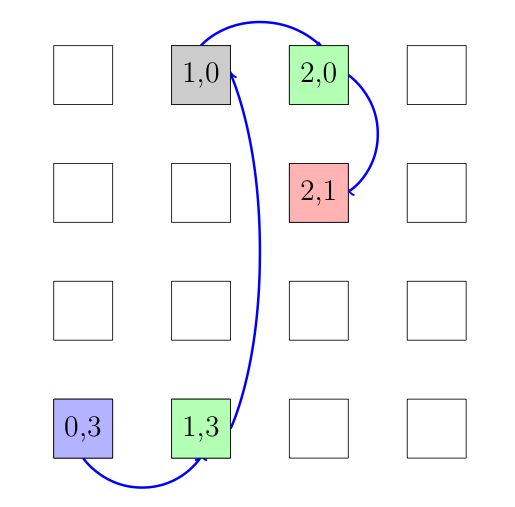
\includegraphics[width=0.5\textwidth]{figures/tikz/hypercube/hypercube_valiant.png}
\caption{Valiant routing within a hypercube.  Packet travels from blue to red via a random intermediate destination shown in gray. Additional intermediate switches are shown in green.}
\label{fig:topologies:hypercubeValiant}
\end{figure}
